\section{Introduction to Saturnin}
\subsection{Saturnin Basics}

\begin{frame}{Saturnin Cipher Basics}
\begin{itemize}
    \item \textbf{Saturnin} is a symmetric \alert{block cipher} designed with post-quantum security and lightweightness in mind.
    \item Key features:
    \begin{itemize}
        \item \textbf{256-bit state} and \textbf{256-bit key}.
        \item Lightweight design suitable implemented using bitsliced operations.
        \item Structured similarly to AES, but uses a 3D 4x4x4 \alert{nibble cube} state.
    \end{itemize}
    \end{itemize}

\end{frame}


\subsection{Post Quantum Motivation}
\begin{frame}{Why Post-Quantum Ciphers?}
\begin{itemize}
    \item Quantum algorithms such as \textbf{Shor's algorithm} threaten asymmetric schemes (RSA, ECC).
    \item Symmetric ciphers are more resistant, but:
    \begin{itemize}
        \item Grover's algorithm reduces brute-force cost from $2^n$ to $2^{n/2}$.
        \item Hence, to maintain $\sim 2^{128}$ security, block ciphers need \textbf{at least 256-bit keys/states}.
    \end{itemize}
    \item Research into \alert{lightweight, quantum-safe symmetric ciphers} is therefore ongoing.
\end{itemize}
\end{frame}

\subsection{Why the name Saturnin?}
\begin{frame}{Why the name Saturnin?}
    Saturnin the Duck. The duck is undeniably a symbol of lightness because it floats. It has been famously used as the reference for lightness throughout the ages. Saturnin the duck is the most famous duck in France.
    \\
    Kepler found the distance between the five known planets to be calculated by inscribing each Platonic solid inside a sphere. And saturn got associated with the cube.
    \begin{center}  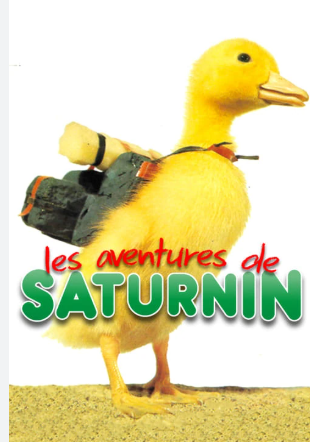
\includegraphics[width=0.55\textwidth,height=0.6\textheight,keepaspectratio]{Images/Figures/duck.png}
    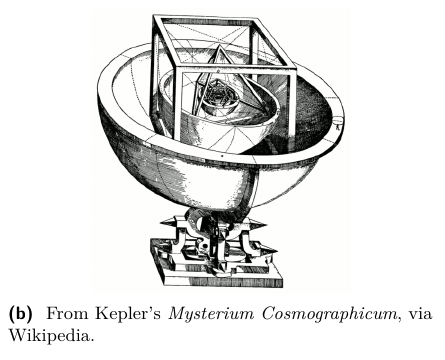
\includegraphics[width=0.55\textwidth,height=0.6\textheight,keepaspectratio]{Images/Figures/kepler.png}
    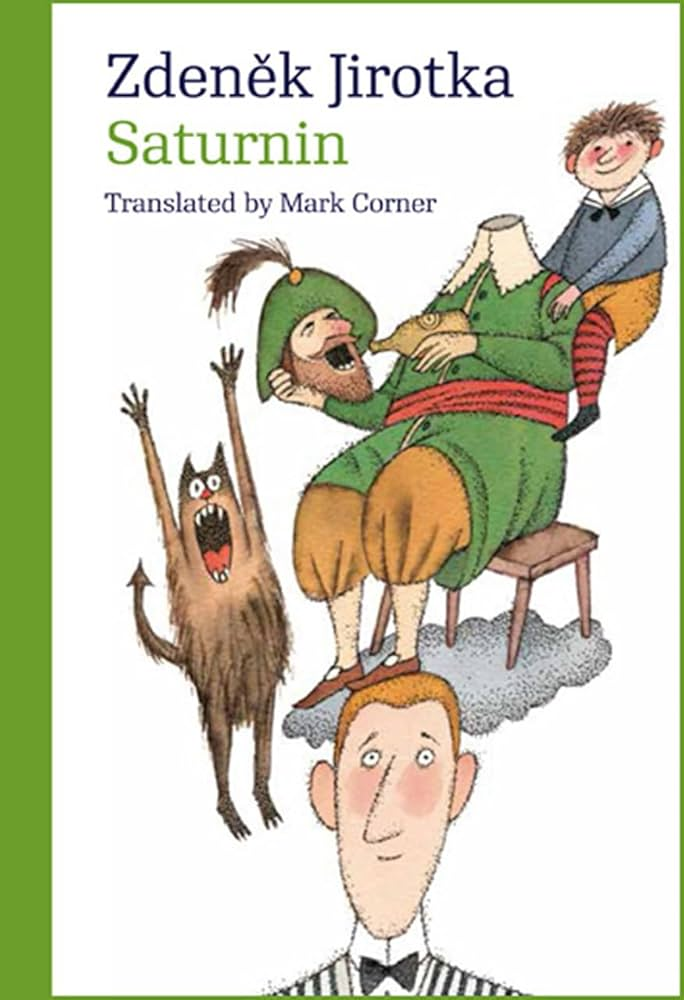
\includegraphics[width=0.55\textwidth,height=0.6\textheight,keepaspectratio]{Images/Figures/novel.jpg}
    \end{center}
\end{frame}



